\chapter{ Validación Experimental}

En este capítulo se detallan tanto los contenidos académicos construidos sobre la herramienta como las diferentes pruebas y experimentos que se utilizaron para probar y verificar la ``Ejecución Mixta'' y sus capacidades. Además de los experimentos, se describirá también su contexto y la relación de cada uno con lo que se quería probar, además de los resultados obtenidos.

\section{Contenidos Académicos de Pruebas}

Para probar y validar toda la implementación, se construyeron una serie de ejercicios con contenido académico que se sirven desde la aplicación remota y se apoyan en el proceso de ``Ejecución Mixta'' para los 3 supuestos de su diseño: \textit{hardware} integrado en el equipo del cliente (cámara), simulación local y \textit{hardware} externo (robots reales).

\subsection{Ejercicio del Filtro de Color}

Dado el origen de la idea de este TFM, resulta lógico que la temática del primer ejercicio tuviese que ver con la visión artificial. El cuadernillo define un ejercicio consistente en un sencillo filtro de color, una de las tareas más simples de la visión artificial que suele aparecer en todo proyecto de robótica que involucre cámaras. El objetivo del mismo es hacer el \textit{tracking} de un objeto de la imagen en base a cierta propiedad, en este caso su color, para obtener su posición en cada fotograma proporcionado por la fuente de vídeo. Se desarrolló por tanto una plantilla de ejercicio basado en un bucle de iteraciones con intervalo variable (en función de la duración de ejecución de un ciclo) que permite al usuario colocar su código y que éste se comporte de manera cíclica, con una serie de métodos a su disposición para facilitar el proceso de desarrollo de su código como parar, restablecer o ejecutar la lógica.

El primer reto a resolver es el acceso a la fuente de imágenes, también como parte de esta infraestructura del ejercicio. Sea cual sea la naturaleza del servidor de vídeo (un fichero estático almacenado en el sistema de archivos, un dispositivo de vídeo integrado o un sensor de vídeo conectado al equipo a través de USB) es necesario solventar el acceso al \textit{hardware} del cliente web. Para el caso concreto de los sensores de imagen existe mucha funcionalidad resuelta que ya permite acceder a los dispositivos de vídeo detectados en el sistema anfitrión, que se puede obtener a través de \textit{plugins} de ROS o incluso haciendo uso de funciones empaquetadas en OpenCV. Cabe mencionar que éstos métodos solucionan el acceso nativo y que el puente Docker se encarga hacer que esa información esté disponible para el \textit{kernel} de Jupyter. Se optó por ambas herramientas para implementar una fuente de vídeo configurable y así abrir la posibilidad de seleccionarla de entre las opciones antes propuestas.

Una vez conectado el código al flujo de vídeo, se continuó con la infraestructura de soporte del filtro de color que incluye funcionalidad gráfica de visualización que ayuda al estudiante a depurar su código mediante el envío de las imágenes crudas y procesadas por canales WebSockets, módulos de control de flujo para controlar la ejecución iterativa del código y poder implementar algoritmos reactivos y métodos con funcionalidad específica resuelta para poder trabajar en la solución al ejercicio que se ofrecen a través de un API de ejercicio al usuario.

Todo ello se ubica en la ``Ejecución Mixta'' como una aplicación auxiliar que se ejecuta como un agente de la capa de Bajo Nivel dentro del contenedor, y que aportaría la opacidad que se perseguía de cara a que el usuario no lidiase con problemas asociados al \textit{hardware} y al bajo nivel, sino que dispusiese de las imágenes de su fuente a través de una sencilla instrucción en su código, y pudiese trabajar con ellas y visualizarlas con la misma facilidad.

Para terminar con la construcción del primer ejercicio, se implementó una solución de referencia al mismo con una posible vía para obtener el resultado esperado, principalmente haciendo uso de las librerías OpenCV para el tratamiento digital. Aunque los algoritmos planteados para los ejercicios no son objeto de esta tesis, se describe brevemente a continuación el funcionamiento del filtro propuesto:

\begin{center}
Ante la imagen de entrada
\end{center}
\begin{figure}[!hbtp]  \centering\noindent
    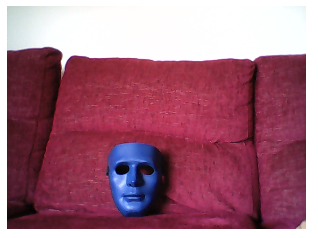
\includegraphics[width=0.65\textwidth]{figures/cf_input.png}
    \caption{Input: Fotograma de la Fuente de Vídeo}
    \label{input}
\end{figure}

Se aplica, en primer lugar, un suavizado a la imagen de entrada con un filtro Gaussiano para eliminar o reducir el posible ruido y, con él, los falsos positivos en el filtro. Luego se convierte el espacio de color de la imagen de entrada, típicamente RGB o BGR, al espacio HSV, donde resulta mucho más sencillo establecer límites para el filtrado de determinado color dado que esta característica se encuentra completamente representada en la componente H, además de ser un espacio mucho más robusto a los cambios en intensidad de luz. Por último, se aplican los límites para obtener una imagen umbral binaria en la que los píxeles de la imagen de entrada cuyo valor de la componente H está entre las cotas establecidas quedan reflejados en la imagen B/N como píxeles de primer plano (de valor 255), y el resto de píxeles se etiquetan como píxeles de fondo (de valor 0).

Para señalar el objeto que supera el filtro, bastaría con hacer una aproximación rectangular a los contornos del objeto blanco de la imagen umbral (detectados en aquellas regiones en las que la derivada es muy grande, cambios rápidos de píxeles blancos a negros). Se escoge el contorno más grande localizado para asegurar la identificación de todo el conjunto de píxeles que forman el objeto. Se pueden aplicar otras técnicas para mejorar el filtrado y eliminar ruido, como operaciones morfológicas o técnicas de post-procesado.
\begin{figure}
\centering
\begin{subfigure}{.32\textwidth}
  \centering
  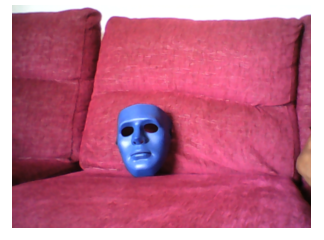
\includegraphics[width=.95\linewidth]{figures/cf_smooth.png}
  \caption{Suavizado de la Imagen}
  \label{smooth}
\end{subfigure}
\begin{subfigure}{.32\textwidth}
  \centering
  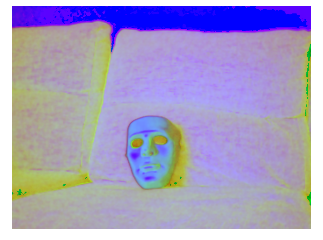
\includegraphics[width=.95\linewidth]{figures/cf_hsv.png}
  \caption{Conversión a HSV}
  \label{hsv}
\end{subfigure}
\begin{subfigure}{.32\textwidth}
  \centering
  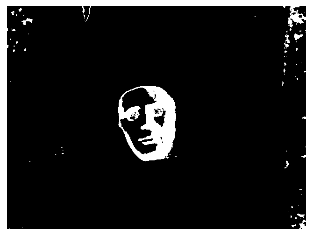
\includegraphics[width=.95\linewidth]{figures/cf_mask.png}
  \caption{Imagen Umbralizada}
  \label{mask}
\end{subfigure}
\caption{Procesado de Imagen para el Filtro de Color}
\label{procesado}
\end{figure}

El proceso descrito se muestra gráficamente en la Fig. \ref{procesado}. De esta manera, nuestro cuadernillo de Jupyter relleno incluye ya la lógica que resuelve el filtro, además del recubrimiento de código auxiliar que hemos comentado y que contiene el \textit{back-end} del ejercicio con los métodos de acceso a la fuente de vídeo, de recogida de imágenes, de visualización y control, etc. En la interfaz de Jupyter se pueden mostrar en todo momento las imágenes que reflejan el estado del proceso a través del API de programación de ejercicio y varias librerías gráficas (entre ellas OpenCV y matplotlib), como se ve en la Fig. \ref{ui_cf_jupyter}.

\begin{figure}[!hbtp]  \centering\noindent
    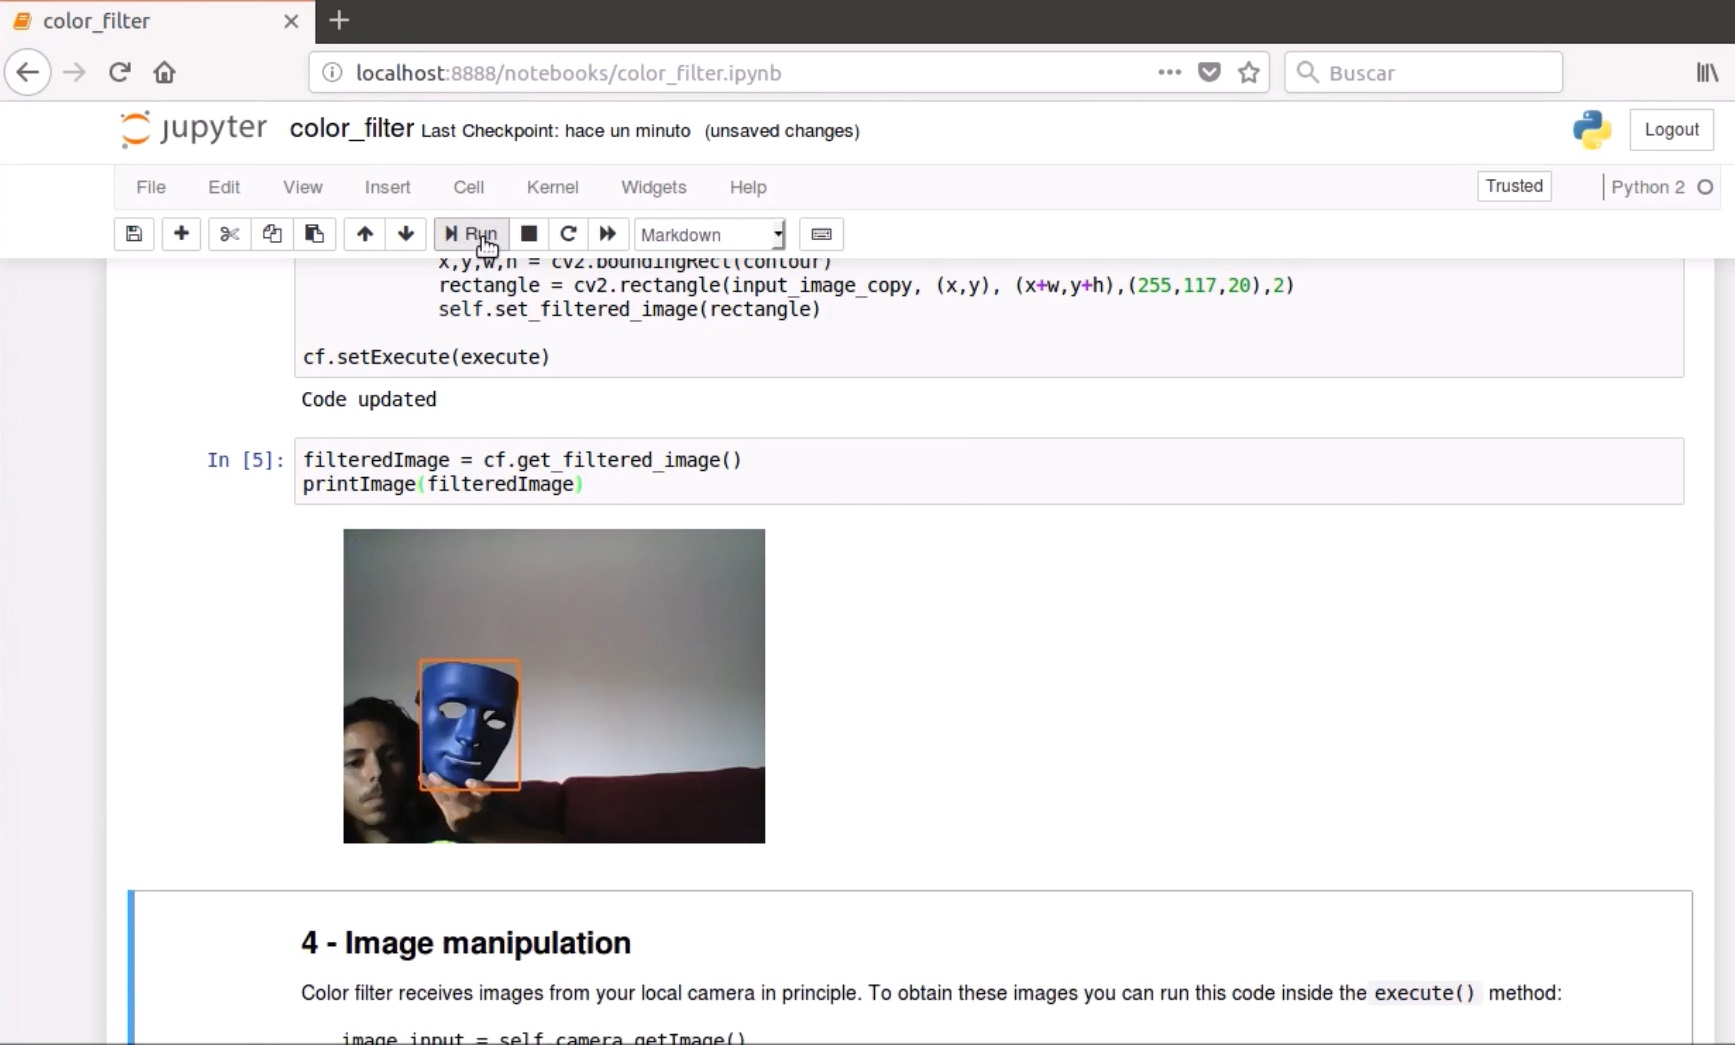
\includegraphics[width=0.99\textwidth]{figures/ui_cf_jupyter.jpg}
    \caption{UI de Jupyter para el Filtro de Color}
    \label{ui_cf_jupyter}
\end{figure}

Se puede encontrar un vídeo mostrando el funcionamiento de este ejercicio en el siguiente enlace:

\textbf{Ejercicio del Filtro de Color}

\url{https://www.youtube.com/watch?v=QnhI0jsEtp4}

\subsection{Ejercicio del Sigue Líneas con Fórmula 1}

Este ejercicio, consistente en el clásico Sigue Líneas de la robótica, permite validar experimentalmente el mecanismo de simulación. Se trata de conseguir que un robot simulado con Gazebo, en este caso un Fórmula 1, procese las imágenes obtenidas con su cámara delantera para detectar una línea de determinado color e implementar un controlador que le permita seguirla.

La infraestructura de este ejercicio queda también recogida en un fichero de \textit{back-end} que dispone, de manera similar al ejercicio anterior, un API de utilización del ejercicio que permite, en este caso, actuar sobre la simulación, es decir, acceder a las interfaces de actuación y sensorización del robot simulado y detener, pausar y reanudar la ejecución del código. Esta estructura de ejercicio incluye la disposición de los canales de ROS de intercambio de información entre Jupyter y el simulador, como ya se mostró en el capítulo anterior.

Para resolverlo se realiza una sencilla segmentación basada en el color para obtener la línea de la imagen, aplicando un filtro y operaciónes morfólogicas de cierre y erosión para eliminar los falos positivos. El resultado del procesado es similar al siguiente:

\begin{figure}[!hbtp]  \centering\noindent
    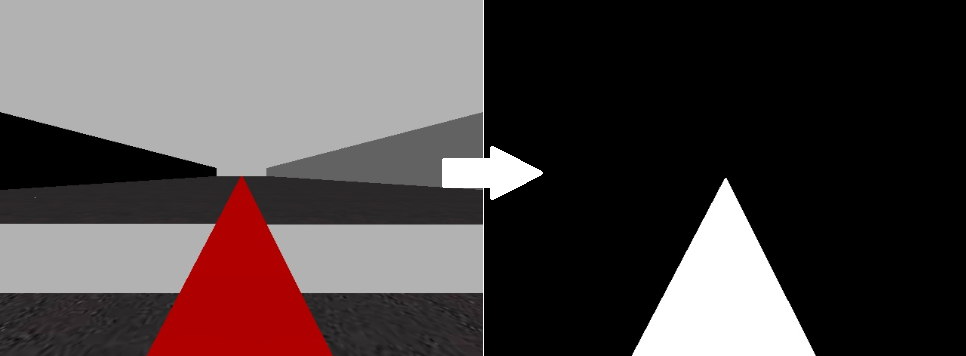
\includegraphics[width=0.99\textwidth]{figures/fl_process.png}
    \caption{Procesado de la imagen del F1}
    \label{fl_process}
\end{figure}

De esta imagen resultante se obtiene el píxel central de la línea de la última fila de la misma, y con él se estiman las coordenadas en las que se encuentra dicho centro, objeto de seguimiento. Luego se implementa un sencillo control basado en la desviación entre la posición actual y la posición objetivo (Listing. 5.1)

\begin{minted}[
    gobble=4,
    frame=single,
    linenos
  ]{python}
    if (deviation == 0):
         self.motors.sendV(3)
    elif (right_pixel_position[0] == 1000):
         self.motors.sendW(-0.0000035)
    elif ((abs(deviation)) < 85):
         if ((abs(deviation)) < 15):
             self.motors.sendV(1)
         else:
             self.motors.sendV(3.5)
         self.motors.sendW(-0.000045 * deviation)
    elif ((abs(deviation)) < 150):
         if ((abs(deviation)) < 120):
             self.motors.sendV(1)
         else:
             self.motors.sendV(1)
         self.motors.sendW(-0.00045 * deviation)
    else:
         self.motors.sendV(1)
         self.motors.sendW(-0.0055 * deviation)
\end{minted}
\begin{lstlisting}[caption=Control basado en desviación]
\end{lstlisting}

Un ejemplo del uso de este ejercicio se puede encontrar en el siguiente enlace:

\textbf{Ejercicio del Sigue-Líneas con Fórmula 1}

\url{https://www.youtube.com/watch?v=39MVVn3u8SE}

\subsection{Ejercicio del Cuadrado con el dron Tello Real}

Ese ejercicio se trata de realizar el más simple control de un robot real para que dibuje un cuadrado. En este caso, se utilizará un dron real que deberá despegar y aterrizar en el mismo sitio, después de haber completado las aristas de un cuadrado como recorrido.

El interés de este ejercicio radica en la inclusión al mecanismo de un \textit{driver} para un robot real, en este caso un \textit{driver} casero para el robot Tello (Listing. 5.2), un cuadricóptero de DJI e Intel cuyo precio de mercado está al alcance del consumidor medio. El uso de este \textit{driver} permite validar la funcionalidad asociada a robots reales de la ``Ejecución Mixta'', en la que al acceso a las interfaces del robot real no se haría a través de ROS, sino mediante el driver implementado. Una vez construido el \textit{driver} en lenguaje Python, se creó un paquete PIP con el objetivo de poder utilizarlo desde el código del usuario, el cual lo importa como una librería normal y corriente y accede a sus funciones y métodos públicos para controlar el dron (Listing. 5.3). 

\begin{minted}[
    gobble=4,
    frame=single,
    linenos
  ]{python}
    #!/usr/bin/env python
    # -*- coding: utf-8 -*-
    
    import socket, threading, time, libh264decoder, cv2
    import numpy as np
    from math import pi as PI
    from speed_thread import SpeedThread
    
    MAX_VEL = 1.5 # m/s
    MIN_VEL = 0.1 # m/s
    MAX_ROT_VEL = 1 # deg/s
    MAX_ROT_VEL = 360 # deg/s
    ORANGE_MIN = np.array([117, 239, 76],np.uint8)
    ORANGE_MAX = np.array([179, 255, 255],np.uint8)
    
    class Tello:
        """Wrapper class to interact with the Tello drone."""
        def __init__(self, local_ip, local_port,
        command_timeout=.2, tello_ip='192.168.10.1',
                     tello_port=8889):
            # vels vector
            #   [
            #       Right(+)/Left(-),
            #       Forward(+)/Backward(-),
            #       Up(+)/Down(-),
            #       Yaw_right(+)/Yaw_left(-)
            #   ]
            self._vels = [0, 0, 0, 0]
            self.abort_flag = False
            self.decoder = libh264decoder.H264Decoder()
            self.command_timeout = command_timeout
            self.response = None  
            self.frame = None  # numpy array BGR
    
            # socket for sending cmd
            # -------------------------------------------
            self.socket = socket.socket(socket.AF_INET,
                                        socket.SOCK_DGRAM)  
            self.tello_address = (tello_ip, tello_port)
            self.socket.bind((local_ip, local_port))
            # -------------------------------------------
    
            # thread for speed control
            # -------------------------------------------
            self.kill_event = threading.Event()
            self.speed_thread = SpeedThread(self)
            # -------------------------------------------
    
            print("Conectando con Tello .....")
            # to receive video -- send cmd: command, streamon
            self.socket.sendto(b'command', self.tello_address)
            print ('[Tello] Preparando controlador')
            self.socket.sendto(b'streamon', self.tello_address)
            print ('[Tello] Preparando flujo de vídeo')
    
            # [...]
\end{minted}
\begin{lstlisting}[caption=Snippet del Driver de Tello]
\end{lstlisting}

\begin{minted}[
    gobble=4,
    frame=single,
    linenos
  ]{python}
    from tello.tello_wrapper import Drone
    tel = Drone('', 9005)
\end{minted}
\begin{lstlisting}[caption=Uso del Driver]
\end{lstlisting}

Este \textit{driver} actúa como aplicación auxiliar dentro del contenedor de ``Ejecución Mixta'' que es lanzada por el secuenciador y añadida al mecanismo interno de paso de mensajes en un canal concreto, de tal manera que se consigue conectar el código que se ejecuta en Jupyter con el propio robot a través de la red interna.

En cuanto al algoritmo que permite solucionar el ejercicio, se trata simplemente de utilizar las funciones de control por posición incluidas en el \textit{driver} implementado con los valores concretos de medida de la arista y ángulo de giro de 90º.

Se puede ver el funcionamiento de este ejercicio en el siguiente vídeo:

\textbf{Ejercicio del Cuadrado con el dron Tello}

\url{https://www.youtube.com/watch?v=4GVvF_ce6Ko}

\section{Experimentos con el Servidor en Producción}

Además de las pruebas realizadas con la plataforma que se servía de manera local, durante el desarrollo también se montó un entorno de pruebas sobre un servidor alojado en la universidad con un dominio accesible.

La motivación de ésta prueba es demostrar el funcionamiento compartido de la herramienta, y verificar que no existe barrera alguna en lo relativo a la ubicación física del cliente y del servidor de ``Ejecución Mixta'' y su \textit{hardware} a controlar. Se puede validar también la capacidad de atravesar NATs y \textit{firewalls} a través de Internet, además de los frecuentes problemas de origen cruzado de los protocolos de intercambio de datos. Se plantea por último el escenario para probar el enlace entre una aplicación robótica de naturaleza remota y el motor local de ``Ejecución Mixta'`.

Se analizaron los parámetros críticos relacionados con la comunicación a través de Internet desde distintos puntos de acceso (nacionales) y con máquinas de distintos rangos operacionales y distintas restricciones de acceso a la red. Los resultados se recogen en la tabla \ref{tabla:pros_cons}.

\begin{table}[htbp]
\begin{center}
\begin{tabular}{| p{1.8cm}| p{2.6cm} | p{1.7cm}| p{2.4cm}| p{3cm}|}
\hline
Navegador & Funcionamiento & Latencia & Ancho de Banda Consumido & Tiempo de Establecimiento de Comunicación \\
\hline \hline
Chrome & 100\% & 38 ms & 0.24 Mbps & 2.8 s\\ \hline
FireFox & 100\% & 36 ms & 0.23 Mbps & 3.1 s\\ \hline
Opera & 100\% & 40 ms & 0.24 Mbps & 3.5 s\\ \hline
Safari & 100\% & 38 ms & 0.28 Mbps & 2.9 s\\ \hline
Internet Explorer & 100\% & 44 ms & 0.13 Mbps & 4.2 s\\ \hline
\end{tabular}
\caption{Tabla de Resultados de Parámetros de Red.}
\label{tabla:pros_cons}
\end{center}
\end{table}

De la tabla de parámetros resultantes se deduce que el funcionamiento es indiferente del navegador elegido, con mejor o peor desempeño en función de la conexión de red, y de la eficiencia de la tecnología de computación del propio navegador. Se puede ver que la latencia media no es crítica, permitiendo un uso fluido de la herramienta en la web, y que en términos de ancho de banda el consumo es prácticamente equivalente al que se obtiene siendo cliente de un servicio de VOD, vídeo bajo demanda. Se demuestra con todo lo anterior que la herramienta de ``Ejecución Mixta'' está preparada para funcionar como parte de cualquier servicio con capacidad de recursos normal a través de la web.

\section{Experimentos de uso con Estudiantes de Prueba}

Para no limitar las pruebas a un único entorno cliente se reunió un conjunto de usuarios que accedieron a hacer las funciones de \textit{betatesters} de manera voluntaria, lo que permitió ampliar el ámbito de experimentación y el alcance de las pruebas, además de su validez sustentada en la generalización, en medias aritméticas de las capacidades y en porcentajes de éxito y fracaso.

Cabe destacar que cada sujeto de pruebas disponía de su propio entorno, es decir, de su máquina con ciertas prestaciones y cierto sistema operativo a cargo. Los \textit{betatesters} tenían mayoritariamente distintas distribuciones de Linux y, en algunos casos, versiones de Windows. En la mayoría de los casos el cliente no disponía de instalación previa de ninguna de las herramientas de las que hace uso la ``Ejecución Mixta'' en su sistema, y ningún cliente disponía de todas ellas.

\begin{table}[htbp]
\begin{center}
\begin{tabular}{| p{1.8cm}| p{2.6cm} | p{1.7cm}| p{2.4cm}| p{3cm}|}
\hline
Modalidad & Funcionamiento & Eficiencia & Carga media en Servidor & Carga media en Cliente \\
\hline \hline
Simulación & 100\% & 60\% & 15\% & 85\%\\ \hline
Cámaras locales integradas & 100\% & 80\% & 10\% & 90\%\\ \hline
Robots Reales & 80\% & 95\% & 0.5\% & 99.5\%\\ \hline
\end{tabular}
\caption{Tabla de Resultados de Sujetos de Pruebas.}
\label{tabla:res_pruebas}
\end{center}
\end{table}

Se observa en la tabla \ref{tabla:res_pruebas} que la totalidad de los usuarios pudieron acceder a la simulación a través de la aplicación derivando el cómputo a su propia máquina a través de la herramienta implementada. La eficiencia en este caso estuvo supeditada al \textit{hardware} del que el cliente disponía para hacerse cargo de la ejecución, especialmente del \textit{hardware} de aceleración gráfica. En todos los casos se experimentó un uso razonablemente bueno.

En cuanto al desempeño de la herramienta en conjunto con los sensores de visión integrados en la máquina del cliente se consiguió que funcionase para todos los sujetos. En este caso se liberaba de algo más de carga al servidor dado que la tasa de refresco de imágenes era más baja que la de la escena de simulación. Se comprobó que el procesado de imágenes que se intercambian por Internet es posible sin sufrir consecuencias temporales gracias al énfasis de la carga en el lado cliente. El acceso a las cámaras se garantizó en los sistemas operativos probados.

Hubo una cantidad menor de pruebas realizadas frente a robots reales dada su escasez. No se consiguió funcionar en los SO basados en Windows dado que ningún usuario disponía de las versiones para las que Docker ofrece soporte. En el caso de los basados en Linux la eficiencia fue máxima, además del grado de explotación de la herramienta, que si bien nació para soportar la ejecución local de algoritmos de visión artificial, parece tener mayores ventajas para el caso de uso de los robots. 

Se infiere de lo anterior que la relación eficiencia-prestaciones fue en todos los casos al menos ligeramente positiva, y que la ``Ejecución Mixta'' funciona siempre para todos los supuestos para los que da soporte.

